\chapter{Bezpečnosť SCADA systémov}
\label{bezpecnost}
\tab Počítačové útoky sú v dnešnej dobe skutočnou hrozbou. Jedným z hlavných dôvodov ohrozenia SCADA systémov je ich postupný prechod na IP vrstvu. Systémy sa stále rozrastajú a vzdialenosť jednotlivých koncových staníc od riadiacej je čoraz väčšia, čo znemožňuje systému komunikovať na fyzickej vrstve. Je preto potrebné vytvoriť komunikačný kanál (napr. VPN spojenie), na vzdialené monitorovanie, medzi jednotlivými stanicami. Na jednej strane je to užívateľsky veľmi prívetivé, je možné vzdialene sledovať a riadiť veľmi veľké množstvo zariadení. Taktiež je možné centrálne vykonávať rôzne aktualizácie ap. Avšak vytvorenie komunikačného kanálu v značnej miere zjednodušuje útočníkom napadnúť a infikovať danú sieť, nakoľko komunikačný kanál môže byť použitý ako zadný vchod (backdoor) do systému. Preto je potrebné komunikáciu v sieti neustále monitorovať (flow monitorovanie) a mať k dispozícií nástroje (rôzne sondy ap.), ktoré sú schopné zachytiť neštandardnú komunikáciu v sieti a včas varovať pred bezpečnostným incidentom. Dôsledky jednotlivých incidentov sa môžu pohybovať od relatívne malých, ako je napríklad prerušenie prebiehajúcej operácie alebo zmena operačného procesu po veľké, ako úmyselné sabotáže s cieľom spôsobiť systému citeľnú ujmu. Jednotlivé útoky nemusia mať vplyv iba na systém samotný, ale aj na okolitú spoločnosť. Napríklad útoky na veľké komplexy ako elektrárne, rafinérie, čističky môžu mať veľký dopad aj na životné prostredie (únik ropy, uvoľnenie toxických látok). Niektoré útoky môžu mať dokonca za následok zranenia alebo straty na životoch, potencionálne katastrofické výbuchy ap\cite{Security}. \par
Úspešný útok môže mať mnoho rôznych následkov zahŕňajúc:
\begin{itemize}
\item zmeny alebo blokovanie zamýšlaného procesu, napr. zmeny v zamýšlanom množstve vyrobenej el. energie,
\item zmeny, oneskorenie alebo blokovanie v infomácií o nameraných hodnotách, veľký dôsledok môže mať napríklad pri obchodovaní s energiami,
\item neautorizované zmeny v inštrukciách, prípadné vypnutie jednotlivých zariadení ako generátory.
\end{itemize}
Konečným dôsledkom útoku môže byť čokoľvek od finančnej straty až po stratu fyzického zabezpečenia systému s dopadom na okolný ekosystém, miestnu komunitu, prípadne dokonca aj štát. Stručný prehľad dopadu útokov rôznych veľkostí je na obrázku \ref{attackcons}.
\begin{figure}[h]
    \centering
    \scalebox{0.55}{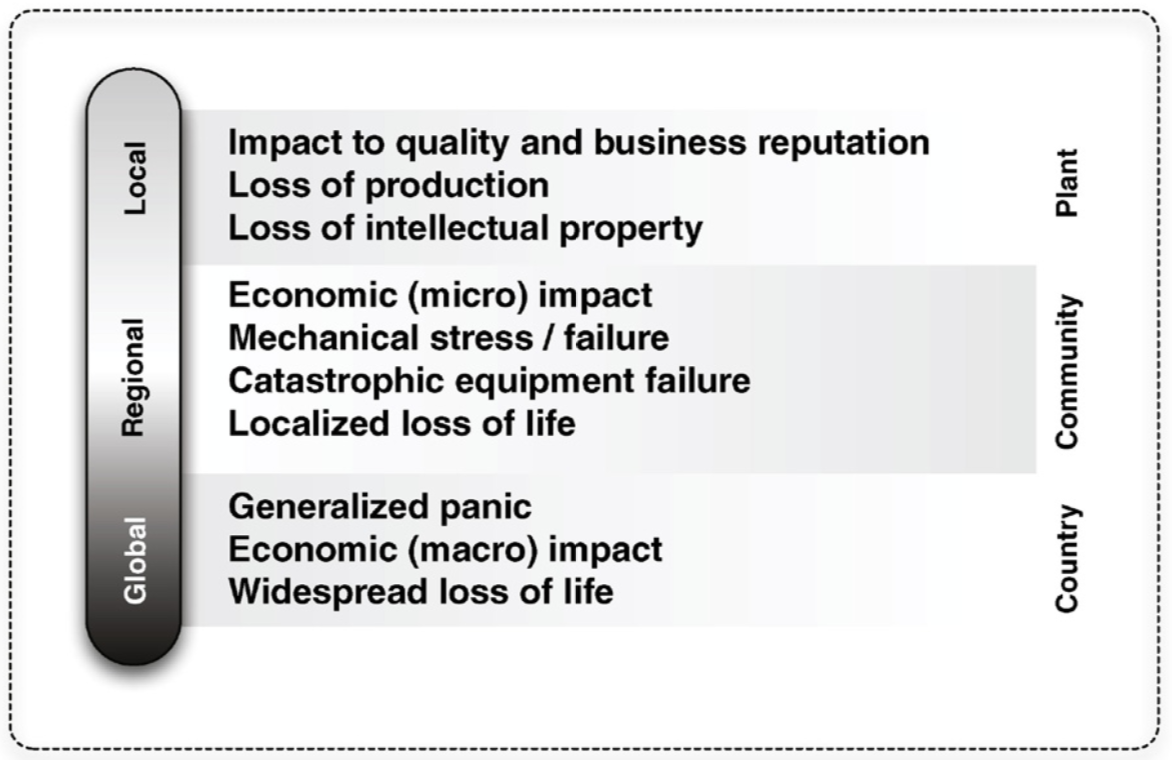
\includegraphics{security_impact}}
    \caption{Dopad rôznych druhov útokov\cite{Security}}
\label{attackcons}
\end{figure}

\section{Bezpečnostné riziká}
\tab Pri posudzovaní bezpečnosti a bezpečnostných rizík v SCADA systémoch sa rozlišuje medzi dvoma typmi útokov. Útoky cez SCADA kanále (SCADA channels) a útoky cez podporné kanále (maintenance channels)\cite{Security}. \par
SCADA kanále sú komponenty slúžiace na primárne účely SCADA systémov - zber a prenos dát, skladovanie a spracovanie údajov a informácií z komunikácie medzi jednotlivými komponentami systému. Medzi typické komponenty SCADA systémov patria:
\begin{itemize}
\item Systém riadenia distribúcie - súbor aplikácií na sledovanie a riadenie systému
\item SCADA servery
\item Vzdialené koncové zariadenia
\item Inteligentné meracie zariadenia
\item Ochranne články
\end{itemize}
Podporné kanále sú systémy slúžiace na inštaláciu a údržbu vyššie spomenutých súčastí systému. Taktiež slúžia na sprostredkovanie komunikácie medzi nimi. Typicky to sú:
\begin{itemize}
\item Inžinierske stanice
\item Spúšťacie (commissioning) servery
\item Servery na synchronizáciu času v systému
\item Monitorovacie a logovacie servery (SNMP, syslog)
\end{itemize} \par
Hlavným dôvodom rozlišovania medzi jednotlivými súčasťami systému je to, že každý so sebou nesie rozličné bezpečnostné riziká. Komunikácia cez SCADA kanály je väčšinou typu počítač-počítač a prenašajú sa iba prevádzkové data, nie konfiguračné zmeny alebo binárky. Narušenie alebo zneužitie sa v monitorovanej komunikácií dá ťažko skryť. To znamená, že je väčšina útokov relatívne rýchlo detekovateľná. Avšak pri podporných kanáloch je to o niečo komplikovanejšie. Autorizované zmeny na jednotlivých komponentoch vykonané pracovníkom spoločnosti sa moc nelíšia od neautorizovaných zmien vykonaných útočníkom. A pretože podporné služby vyžadujú privilegovaný prístup do systému, je to veľmi lákavé pre útočníkov, ktorí chcú získať permanentnú kontrolu nad systémom. Je ale možné spoľahlivo monitorovať aj túto časť siete, avšak iba ak sa všetky podporné procesy vykonávajú "disciplinovane". \par
V počítačových sieťach obecne existuje mnoho rôznych druhov útokov. Avšak pri SCADA systémoch sa väčšina z nich neberie do úvahy, nakoľko je pri nich predpoklad dostatočného zabezpečenia systému a dôkladná konfigurácia firewallov na prepúšťanie iba najdôležitejšej komunikácie. To znamená, že očividné "diery"\ do systému by mali byť uzavreté. Napriek tomu ale zostáva niekoľko typov útokov, ktorými sú SCADA systémy ohrozené\cite{Security}:
\begin{itemize}
\item Útok cez SCADA kanál
\item Útok cez podporu SCADA serverov
\item Útok cez podporu koncových zariadení
\item Útok "zvnútra"
\end{itemize}
Táto práca je zameraná najmä na útoky cez SCADA kanále a cez podporu koncových zariadení.

\subsection{Útoky cez SCADA kanále}
\tab Pri samotnom získavaní prístupu do riadiaceho systému SCADA siete existuje iba niekoľko možností ako ho infikovať. Nakoľko je na prístup do systému vyžadovaná autentizácia, útočníci sa môžu do systému dostať dvoma spôsobmi. Prvý je získanie prístupu cez platné autentizačné údaje niekoho iného. Rozhrania na výmenu údajov cez IT sieť by však mali byť obmedzené na export dát, takže dopad útoku na systém nie je taký veľký. Druhý spôsob je do systému rozšíriť malware cez servery prístupné z IT domén. Ak bude software využívať zraniteľnosti systému, umožní tak útočníkovi robiť veľké zmeny v jadre systému a môže výrazne ovplyvniť a ohroziť celý systém. Pravdepodobnosť úspechu takéhoto útoku výrazne závisí na zabezpečení a počte zraniteľných miest, ktoré systém má. \par
Ďalším vstupným bodom do SCADA systému je útok na koncové stanice. Nakoľko systém väčšinou využíva veľa koncových staníc, niektoré z nich dokonca na odľahlých miestach, ani dobrá fyzická ochrana nemôže plne zabrániť prieniku do zariadenia a následne do systému. Či už ide o fyzický alebo kybernetický útok, takéto útoky väčšinou nespravia v systéme veľké škody, nakoľko ide o napadnutie jedného zariadenia a na ovplyvnenie viacerých by bolo potrebné viesť útok cez riadiacu stanicu. Samozrejme to ale záleží aj od použitej topológie, ktorá je využívaná na prepojenie riadiacej stanice a koncových staníc. \par
Útočníci môžu využiť zariadenia na koncových staniciach na prístup do systému s platnými autentizačnými údajmi, avšak ak je systém dostatočne zabezpečený, môžu nanajvýš posielať nesprávne/podvrhnuté informácie o nameraných hodnotách. Aby boli schopný spraviť väčšie škody, museli by napr. rozšíriť po systéme software, ktorý bude schopný ovládať väčšie množstvo koncových staníc. \par
Ďalší typ útoku je pripojenie do systému cez spojenie s riadiacim strediskom. Sú dva typy hrozieb, ktoré môžu byť takýmto útokom napáchané. Prvý je pripojenie cez vlastnú riadiacu stanicu s jednotlivými koncovými zariadeniami s využitím platných autentizačných údajov. Útočník tak môže napr. posielať neautorizované príkazy jednotlivým staniciam. Druhý útok spočíva vo využití zraniteľnosti systému, čo môže byť zneužité napr. na rozšírenie rôznych typov malware do siete. \par
Keď už útočník prenikne do systému, je schopný využívať jeho plnú funkcionalitu a rôznymi spôsobmi ho tak poškodiť\cite{Security}.

\subsection{Útoky cez koncové zariadenia}
\tab Vybavenie koncových staníc ako RTU (Remote Terminal Units - mikroprocesorom riadené zariadenia) alebo IED (Intelligent Electronic Devices - inteligentné merače) môžu byť väčšinou spravované z jednej centrálnej stanice. Ak útočník dokáže získať prístup k týmto hostom, napr. cez platné autentizačné údaje, môže zmeniť konfiguráciu jednotlivých zariadení. Ak zariadenie nie je konfigurované lokálne, môže byť konfigurované cez nejaké externé zariadenie ako napr. laptop, USB kľúč, pamäťovú kartu ap. To je opäť riziko na rozšírenie malware po sieti. \par
Ďalšia cesta, ako je možné napadnúť systém, je využiť zraniteľnosti jednotlivých zariadení na stanici. Nakoľko väčšinou využívajú normálny IT software, poskytujú tým útočníkom jednoduchú cestu do SCADA systému. Koncové stanice môžu byť napadnuté zo sieťovej strany ale aj cez koncové zariadenia, ak do nich niekto vloží malware, ktorý sa môže ďalej šíriť do siete. \par
Riziko architektúry SCADA systému je aj v tom, že je možné si vytvoriť vstup do systému pripojením vlastného zariadenia. To sa týka najmä koncových staníc, ktoré sú menej chránené ako riadiaca stanica\cite{Security}.
\section{Typy útokov}
\tab Keď sa raz útočník dostane do systému a identifikuje svoj cieľ, existuje mnoho spôsobov, ako ho poškodiť. Medzi najbežnejšie útoky patria:
\begin{itemize}
\item Man-in-the-middle
\item Denial-of-Servise (DoS)
\item Replay útoky
\end{itemize}
Hlavným dôvodom je kombinácia rôznych protokolov a slabá úroveň autentizácie, napr. prenos nezašifrovaných kľúčov po sieti, ktoré sa dajú jednoducho odchytiť a použiť na získanie neoprávneného prístupu do systému. V systémoch, ktoré tvoria spojitosť medzi niekoľkými systémami, ako napr. SCADA server, môže byť trvalá prítomnosť útočníka v riadiacej časti použitá ako základ sekundárneho útoku proti iným častiam siete. Pri takomto útoku je veľmi dôležitý rozdiel medzi ovládnutím cieľa a útokom samotným. Ovládnutie cieľa znamená prístup alebo schopnosť vykonávať s objektom neznámu činnosť. Napríklad spustenie určitého procesu s parametrami nad prípustné medze a tým zariadenie fyzicky poškodiť, prípadne poškodiť viaceré zariadenia, ktoré sú na ovládanom závislé. Útok je na druhej strane schopnosť útočníka vykonávať s cieľovým objektom nežiadúce akcie. V tomto prípade môže zariadenie pracovať, tak ako má, avšak schopnosť napadnúť zariadenie a spôsobiť, že vykoná akciu, ktorú obsluhujúci personál nepožadoval, môže mať negatívne následky. Takéto útoky bývajú spojované s využívaním funkčnosti a zraniteľných miest zariadení. To znamená, že zaslanie riadiacemu zariadeniu príkaz na vypnutie nepredstavuje slabosť zariadenia ako takého, avšak nedostatok overovania a autentizácie umožňuje útočníkovi zaslať nežiadúci príkaz, a tým na istý čas ochromiť systém. Obdobné útoky sú tzv. replay útoky\cite{Security}. \par

\subsection{Man-in-the-middle útok}
\tab Vo svojej práci sa budem najviac zaoberať tzv. útokom man-in-the-middle, ktorý pozostáva z odchytenej a následne zmenej komunikácie medzi dvoma zariadeniami. \par
Pri útoku typu man-in-the-middle sa hovorí o útoku kedy útočník sleduje komunikáciu medzi zariadeniami, odchytáva zasielané správy, mení ich a opätovne zasiela pôvodnému adresátovi. Zariadeniam sa zdá, že medzi sebou komunikujú priamo, avšak v skutočnosti komunikujú cez tretie zariadenie, ktoré ich odpočúva a môže interagovať (zasahovať, meniť zasielané správy). Na obrázku \ref{mitm} je úkažka typickej komunikácie pri útoku man-in-the-middle, spolu so zmenou v zasielanom príkaze. \par
\begin{figure}[H]
    \centering
    \scalebox{0.35}{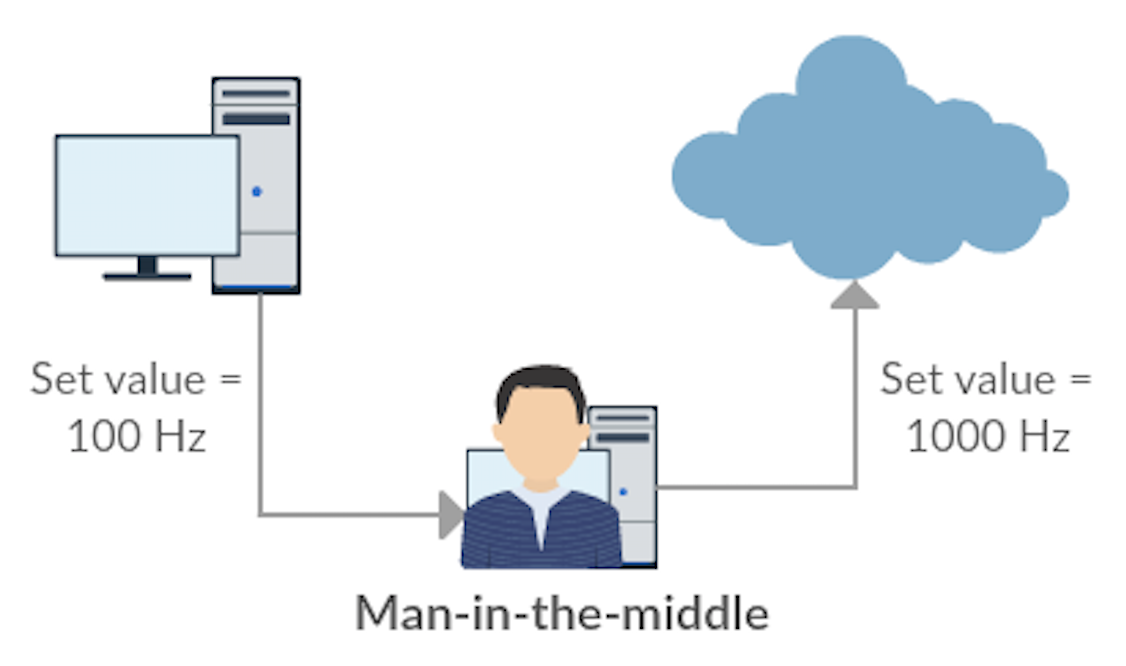
\includegraphics{mitm}}
    \caption{Man-in-the-middle útok}
\label{mitm}
\end{figure}
Ak chce útočník vykonávať man-in-the-middle útok, musí byť schopný zachytiť komunikáciu medzi oboma cieľovými systémami a vložiť do nej nové (upravené) správy. Ak spojenie nemá šifrovanie alebo dokonca ani overovanie autentizáciou, ako je častý prípad pri priemyselnej prevádzke, je man-in-the-middle útok veľmi jednoduchý proces. Avšak aj v komunikáciach, kde sa používa autentizácia, alebo šifrovanie, môže byť stále man-in-the-middle útok úspešný, napr. odpočúvaním kľúčových výmien a prenesením útočníkovho kľúča namiesto legitímneho. Tento spôsob útoku je ale v priemyselných sieťach trochu komplikovaný, nakoľko jednotlivé strany môžu spolu komunikovať dlhú dobu a útočník by musel zneužiť existujúce komunikačné spojenie. Najobtiažnejšou časťou úspešného man-in-the-middle útoku je úspešne prepojiť dátový tok a presvedčiť obe strany, že útočník je skutočne určeným príjemcom jednotlivých správ. Proti tomu je možné sa brániť autentizačnými kontrolami, avšak mnohé priemyselné komunikačné protokoly zasielajú autentizačné údaje v otvorenej podobe, čo uľahčuje útočníkovi prácu, nakoľko mu stačí odsledovať komunikáciu, prečítať autentizačný kľúč a úspešne sa pripojiť do systému\cite{Security}.

\subsection{Denial-of-Service útok}
\tab Denial-of-Service, čiže útok typu odoprenia služby, nastáva, keď sa nejaký útočník snaží odoprieť služby systému pre bežných užívateľov tým, že ho robí nedostupným (neschopným bežnej prevádzky). DoS útoky sú veľmi široká kategória útokov a môže zahŕňať čokoľvek od straty komunikácie so zariadením po narušenie alebo zablokovanie určitých služieb v rámci daného zariadenia (ukladanie, spracovanie I/O). DoS útoky v bežných systémoch väčšinou nemajú veľké následky, ak sú riešené včas. Avšak ak je DoS útok dobre cielený, môže prepnúť dôležité systémy do offline režimu, alebo ich dokonca vypnúť. \par
Automatizované systémy sa nasadzujú na monitorovanie a riadenie rôznych procesov. Tento proces môže ovplyvňovať tok ropy v potrubí, premenú vodnej pary na elektrinu alebo kontrolovať časovač zapaľovania v motore. Strata schopnosti správcu tieto procesy riadiť sa nazýva strata kontroly (Loss of Control - LOC) a zvyčajne vedie k prepnutiu fyzického procesu do "bezpečného"\ stavu vypnutia. To znamená, že aj jednoduché prerušenie kontrolných funkcií môže viesť k fyzickým poruchám na systéme, ktoré môžu pokračovať v odstavení systému, mechanickému zlyhaniu alebo iným katastrofickým scenárom. \par
Oproti DoS útokom na rôzne webové stránky môžu mať priemyselne cielené DoS útoky za následok napr. únik ropy, neplatné šarže výrobkov alebo dokonca explózie. DoS útok v priemyselnom prostredí je oveľa viac ako iba nepríjemnosť a môže viesť k veľmi nepríjemným následkom, ak nebude včas riešený\cite{Security}.

\section{Zaznamenané útoky}
\tab Na rozdiel od IT sietí boli OT siete a komunikácia v nich väčšinou izolované a mali iba minimálnu komunikáciu s inými sieťami. História útokov na priemyselné systémy je preto oveľa menšia ako na IT siete. Avšak útoky na priemyselné systémy môžu mať veľké následky, ktoré môžu spôsobiť stratu na životoch, fyzické poškodenie systému alebo znečistenie okolitého ekosystému. \par
Napríklad na jar roku 2000 sa bývalý zamestnanec istej austrálskej softvérovej spoločnosti uchádzal o zamestnanie v miestnej samospráve, avšak jeho žiadosť bola zamietnutá. Následne sa nespokojnému uchádzačovi podarilo pomocou rádiového vysielača vzdialene získať prístup do kontrolného systému čističky odpadných vôd a zmeniť elektronické údaje pre konkrétne kanalizačné čerpacie stanice. To malo za následok poruchy v prevádzke systému a následné vypustenie viac ako 950 000 litrov odpadných vôd do blízkych riek a parkov, čo malo veľký efekt na miestny ekosystém\cite[p.~3-20]{nist}. \par
V tejto podkapitole bude uvedený prehľad rôznych typov zdokumentovaných útokov na priemyselné IoT siete. 

\subsection{Vlakový signalizačný systém CSX (2003)}
\tab V auguste 2003 bol počítačový vírus Sobig vinený za vypnutie vlakových signalizačných systémov na celom východnom pobreží USA. Vírus infikoval počítačový systém v centrále spoločnosti CSX Corp. v Jacksonville v štáte Florida a vypol signalizáciu, dispečing a iné systémy. Podľa Dana Stessela, hovorcu spoločnosti Amtrak, bolo útokom postihnutých desať vlakov. Vlaky medzi Pittsburgom a Florenciou v Južnej Karolíne boli zastavené kvôli tmavým signálom a jeden regionálny vlak z Richmondu vo Virginií do Washingtonu a New Yorku bol odložený o viac ako dve hodiny. Diaľkové vlaky sa oneskorili o štyri až šesť hodín\cite[p.~3-20]{nist}.

\subsection{Výpadok prúdu v elektrárni v Northeast (2003)}
\tab V auguste 2003 zlyhanie procesoru alarmu v SCADA systéme spoločnosti First Energy zabránilo operátorom riadiacich staníc byť dostatočne informovaní o kritických prevádzkových zmenách v elektrickej sieti. Navyše neúplné informácie o zmenách topológií v systéme zabránili efektívnemu dohľadu nad jeho spoľahlivosťou. \par
Niekoľko kľúčových prenosových 345kV vedení v severnom Ohiu sa zastavilo kvôli kontaktu so stromami. To spustilo kaskádové preťaženie ďalších 345 kV a 138 kV vedení, čo viedlo k nekontrolovanému zlyhaniu celej siete. Celkovo bolo 61 800 MW stratených po zastavení 508 generátorov v 265 elektrárňach\cite[p.~3-20]{nist}.

\subsection{Stuxnet červ (2010)}
\tab Stuxnet bol počítačový červ pre OS Microsoft Windows objavený v júly 2010, ktorý špecificky útočil na priemyselný software a zariadenia\cite[p.~3-20]{nist}. Bol schopný infikovať počítače využívajúce Microsoft Windows od Win2000 po Windows 7 a Windows Server 2008 R2. \par
Ak infikovaný hostiteľ nebol cieľ útoku, ale iba "medzistanica", počiatočná infekcia mohla nahrať rootkit, ktorý automaticky načíta malware pri bootovaní zariadenia a ponechá ho neodhalený kým sa útočník nerozhodne zaútočiť na svoj cieľ z infikovaného zariadenia. \par
Ak infikované zariadenie obsahovalo software Siemens Simatic, existovali metódy využívajúce predvolené poverenia SQL servera, ktoré umožňovali inštaláciu malware do SQL (WinCC). Tiež mal schopnosť prepísať ovládač používaný na komunikáciu s PLC S7 (Programmable Logic Controller) a účinne vytvoriť man-in-the-middle útok, ktorý by umožnil zmenu kódu bežiaceho v PLC bez toho, aby to detekovali používatelia systému.
Stuxnet bol využívaný na prenos užitočnej záťaže nielen pre konkrétne riadiace systémy, ale tiež pre konkrétne konfigurácie riadiacich systémov zahŕňajúc jedinečné čísla modelov PLC a dodávateľov pripojených zariadení. Hľadal konfiguráciu cieľového systému (PLC S7-315-2 / S7-417) a keď bola nájdená, vložil bloky kódu do cieleného PLC, ktorý mohol prerušiť alebo zmeniť prebiehajúce procesy. Stuxnet používal infikované PLC na sledovanie špecifického správania monitorovaním zbernice. \par
Stuxnet mal dva hlavné ciele svojho útoku na užitočnú záťaž:
\begin{itemize}
\item Zvyšovanie a znižovanie rýchlosti centrifugy nad normálne hodnoty. \par
Normálne centrifugy rotujú pri rýchlosti 807-1210 Hz. Po nainštalovaní Stuxnetu, začal monitorovať rýchlosť a veľmi príležitostne zmenil rýchlosť na veľmi rýchlu (1410 Hz), hneď na to na veľmi pomalú (2 Hz) a opäť na rýchle (1064 Hz). To malo za následok fyzické poškodenie súčastí systému.
\item Zvyšovanie tlaku vo vnútri odstrediviek nad normálne hodnoty. \par
Stuxnet taktiež ovlyvňoval tlak vo vnútri odstrediviek. Tento proces zahŕňal uzatváranie tlakových spätných ventilov, ktoré boli počas prevádzky normálne otvorené, čo spôsobovalo nebezpečné zvyšovanie tlaku vo vnútri zariadení\cite{Security}\cite{IoTSec}.
\end{itemize}

\subsection{Útok na ukrajinskú elektráreň (2016)}
\tab Týždeň pred Vianocami v roku 2016 sa podarilo skupine útočníkov napadnúť elektrickú prenosovú stanicu Pivnichna severne od mesta Kyjev a zablokovať dodávku elektrickej energie do časti Kyjeva a priľahlého okolia na jednu hodinu. Útok začal chvíľu pred poľnocou 17. decembra a dodávka elektriny bola obnovená po jednej hodine ráno. \par
Vedúci výzkumu bezpečnosti informačných systémov na Ukrajine Oleksii Yasynskyi povedal, že \textit{útočníci zjavne testovali novú techniku útoku a ich cieľom bolo sabotovať systém.} \par
Pri útoku bol použitý nový nástroj na infikovanie a narušenie prevádzky SCADA systémov - Win32/Industroyer\cite{IoTSec}.
\subsubsection{Win32/Industroyer malware}
\tab Win32/Industroyer je sofistikovaný malware navrhnutý na narušenie prebiehajúceho procesu v zariadeniach SCADA systémov. \par
Industroyed je v súčasnosti veľmi nebezpečná hrozba, nakoľko je schopný priamo ovládať spínače a ističe na elektrických staniciach. Na tento účel používa priemyselné komunikačné protokoly, ktoré sa bežne využívajú v SCADA systémoch. Win32/Industroyer zahŕňa štyri komunikačné protokoly:
\begin{itemize}
\item IEC 60870-5-101
\item IEC 60870-5-104
\item IEC 61850 - Goose
\item OLE na riadenie procesov (Process Control Data Access - OPC DA)
\end{itemize}
Problém v týchto protokoloch je, že boli navrhnuté ešte v časoch, keď bola priemyselná IoT prevádzka izolovaná od bežnej a nebolo možné na ňu zaútočiť z verejnej IP siete. Protokoly preto neboli navrhnuté na podporu bezpečnosti a autentizácie, čo znamená, že útočník v súčasnosti nemusí hľadať zraniteľnosti protokolu, stačí mu vytvoriť malware, ktorý bude komunikovať v danom štandarde. Win32/Industroyer je modulárny malware. Jeho hlavnou zložkou je "zadný vchod"\ (backdoor) do systému, ktorý útočníci využívajú na riadenie útoku: inštaluje a riadi ostatné komponenty a pripája sa k vzdialenému serveru na prijímanie príkazov a reportovanie útočníkovi. \par
Okrem toho implementuje DDoS útok proti špecifickým skupinám ochranných relé, konkrétne sa zameriava na sériu Siemens SIPROTEC. \par
Všeobecne platí, že užitočné zaťaženie funguje v etapách, ktorých cieľom je mapovanie siete a následné prijímanie, a vydávanie príkazov pre konkrétne riadiace komponenty systému, viď obrázok \ref{payload}. \par
\begin{figure}[h]
    \centering
    \scalebox{0.6}{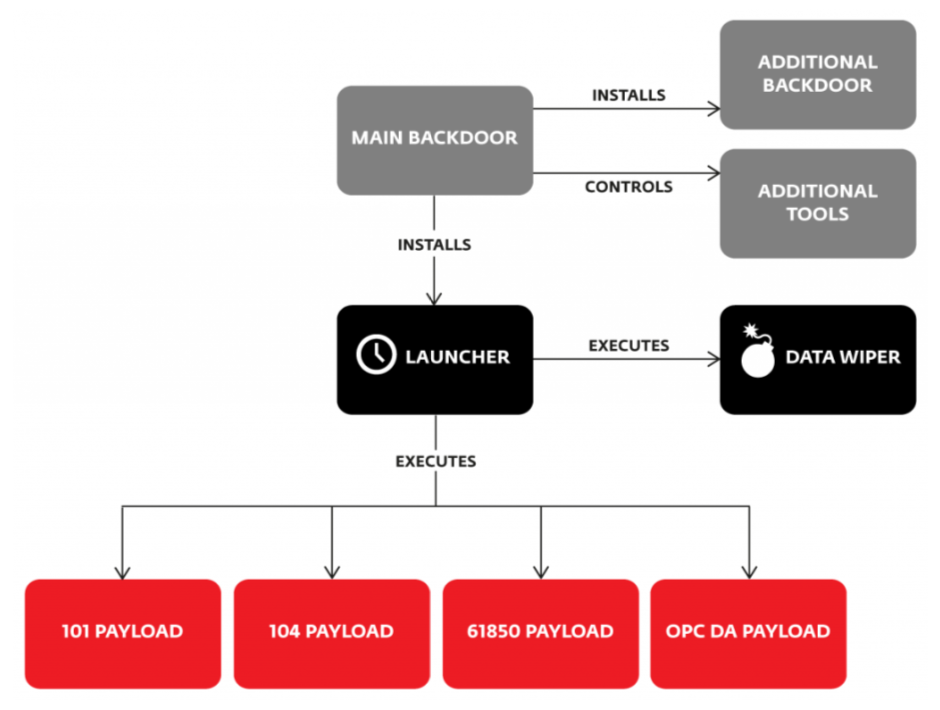
\includegraphics{payload}}
    \caption{Etapy užitočného zaťaženia\cite{IoTSec}}
\label{payload}
\end{figure}
Zadný vchod do systémov celkom priamočiaro spojuje malware so vzdialeným serverom využívajúc HTTPS protokol na zasielanie príkazov od útočníka. Zaujímavé je, že útočníci si môžu nadefinovať špecifickú hodinu, kedy bude tento vchod do systému aktívny, napríklad mimo pracovnej doby. Keď sa vytvorí spojenie so serverom, v {\tt POST} žiadosti sú zaslané jednotlivé údaje\cite{IoTSec}. \par
Je podporovaných niekoľko základných príkazov:
\begin{itemize}
\item 0: spustenie procesu
\item 1: spustenie procesu pod špecifickým užívateľom s patričnými autentizačnými údajmi
\item 2: stiahnutie súboru zo servera
\item 3: zkopírovanie súboru
\item 4: spustenie {\tt shell} príkazu
\item 5: spustenie {\tt shell} príkazu pod špecifickým užívateľom s patričnými autentizačnými údajmi
\item 6: zastavenie
\item 7: zastavenie služby
\item 8: zastavenie služby pod špecifickým užívateľom s patričnými autentizačnými údajmi
\item 9: spustenie služby pod špecifickým užívateľom s patričnými autentizačnými údajmi
\item 10: nahradenie hodnoty registra {\tt image path} pre danú službu
\end{itemize} \par
Pri užitočnom zaťažení komponent protokolu IEC 104 obsahuje konfiguračný súbor pre jednotlivé komponenty IP adresu stanice, cieľový port, ASDU adresu, hodnotu prepínača (zap./vyp.), hodnotu zmeny (0/1) a operáciu (iteračný typ pre IOA: rozsah, sekvenciu alebo posunutie). \par
Po spustení vytvorí vlákno pre každú sekciu staníc definovaných v konfiguračnom súbore. V každom vlákne komunikuje s konkrétnou adresou využívajúc protokol IEC 104. Po vytvorení spojenia s daným zariadením začne zasielať príkazy s ASDU adresou definovanou v súbore kde interaguje s IOA využívajúc SCO (Single command) typ\cite{IoTSec}. \par
Iteračné typy IOA:
\begin{itemize}
\item Rozsah - využívajúc mód rozsahu môže útočník odhaliť všetky dostupné IOA v cielenom zariadení. Protokol IEC 104 štandardne neposkytuje žiadnu obdobnú metódu na získanie takých údajov. \par 
Keď útočník získa potrebný rozsah IOA, môže cez ne začať iterovať a zasielať príkazy {\tt select and execute}, aby mohol zmeniť typ daného IOA a potvrdiť, že patrí do typu SCO. \par
Keď je preiterované cez všetky potrebné IOA, malware začne rozposielať príkazy {\tt select and execute} v nekonečnom cykle, kde postupne zapína a vypína zariadenia.
\item Sekvencia - tento mód môže byť použitý jedine ak útočník vie hodnoty všetkých IOA, ktoré využívajú SCO typ. Malware môže hneď začať nekonečný cyklus v ktorom bude posielať {\tt select and execute} príkazy IOA definovaným v konfiguračnom súbore.
\item Posunutie - je veľmi podobné módu rozsahu. Iteruje sa cez celý rozsah IOA, kde nový rozsah je vypočítaný pridaním hodnoty posunutia k pôvodnej hodnote rozsahu\cite{IoTSec}.
\end{itemize}
\section{Zhrnutie}
SCADA systémy v súčasnosti čelia mnohým rizikám. Je to veľký problém najmä z dôvodu, že systémy sú väčšinou súčasťou kritickej infraštruktúry a útoky na ne môžu mať veľký dopad aj na bežných obyvateľov alebo ekosystém ako taký. Je preto potrebné vedieť útoky včas detekovať a vedieť sa im efektívne brániť. \par
V tejto kapitole bol uvedený základný prehľad bezpečnostných rizík na SCADA systémy spolu s popisom jednotlivých typov útokov. Taktiež bolo uvedených niekoľko príkladov zaznamenaných útokov spolu s dôsledkami, ktoré spôsobili. \par
V ďalšej časti mojej práce budem vychádzať z popisu jednotlivých rizík, ktorým SCADA systémy čelia a vytvorím simulačné prostredie na ich testovanie a sledovanie reakcií systému na ne.




